\section{Grundlagen der Informationsrückgewinnung}
\label{sec:Informationsrückgewinnung}

%In the last decades our world has become more and more interconnected. This interconnection added to the increase of the available bandwidth and the change in business models have forced IT Systems to fulfill its demands, leading to its reorganization into a public utility which offers public services, like water, electricity, etc. The \ac{NIST} defines Cloud computing as "a model for enabling ubiquitous, convenient, on-demand network access to a shared pool of configurable computing resources (e.g., networks, servers, storage, applications, and services) that can be rapidly provisioned and released with minimal management effort or service provider interaction"  \cite{NIST2011}. The Cloud computing model is composed of five characteristics:
	%\begin{enumerate}
	%	\item On-demand self-service: a Cloud user consumes the Cloud provider's computing capabilities automatically without the need of human interaction. 
	%	\item Broad network access: computing capabilities are available via the network and can be accessed using standard mechanisms.
	%	\item Resource pooling: computing capabilities in the Cloud provider side are virtualized to serve multiple consumers simultaneously using a multi-tenant model. The Cloud consumer generally has no sense of the provided resources.
	%	\item Rapid Elasticity: computing and storage resources can be dynamically (and in some cases automatically) provisioned and released to respond to the actual consumers' demand.
	%	\item Measured Service: resources' usage is monitored and measured in a transparent way to the Cloud consumer and provider for control and optimization purposes.
%	\end{enumerate}

%The control that the Cloud consumer has over the computer resources in a Cloud provider infrastructure is defined in three service models: \term{\ac{SaaS}}, \term{Platform-as-a-Service (\ac{PaaS})} and \term{\ac{IaaS}}. \term{\ac{SaaS}} provides to the Cloud consumer access and usage of Cloud provider's applications running on a Cloud infrastructure. The consumer has no control over the underlying infrastructure where the application he uses is deployed. The customer can only control individual application's configurations during his usage of it. \term{\ac{PaaS}} provides the customer with the needed capabilities to deploy applications which's programming language, required libraries, services and tools are supported by the provider. The consumer has no control over the underlying infrastructure where he deploys the application. \term{\ac{IaaS}} is the model which gives most control to the consumer. Thus, the consumer is able to deploy and run arbitrary software and has the control over operating systems, storage and deployed applications, but has no management or control on the underlaying Cloud infrastructure. 

%Although the three service models described above provide both data computation and storage capabilities for the consumer, they do not provide to the customer the possibility to directly and uniquely purchase access of storage services. In this diploma thesis we concentrate in two concrete models: \term{\ac{DBaaS}} and \term{\ac{STaaS}}. Cloud storage providers target a selected number of consumers, who process their data on-premise, but do not  want to cover the expenses of a local database system, or a backup system, among others. The Cloud storage model alleviates the need in organizations to invest in database hardware and software, to deal with software upgrades, and to maintain a professional team for its support and maintenance \cite{dbaasIyer}.  \ac{DBaaS} and \ac{STaaS} can be considered quite similar, except for one of their main distinction characteristics: their access interface. The former is the most robust data solution offered as a service, as it offers a full-blown database functionality. It can be accessed via the most common database protocols, such us MySQL, Oracle, etc, or by REST interfaces supporting \ac{SQL}. Examples of this model are Amazon RDS \cite{amazonrds} and Oracle Cloud \cite{oraclecloud}. On the other hand, the latter provides REST, \ac{SOAP} over \ac{HTTP}, or Web-based interfaces in order to perform the operations over the stored data \cite{cloudstorageWU}. Examples of this model are Amazon Dynamo \cite{amazondynamodb} , Google App Engine Datastore \cite{googleappdatastore}, and Dropbox \cite{dropbox}.

%\ac{NIST} defines four deployment models in Cloud computing. A private Cloud consists in a Cloud infrastructure which is provisioned exclusively for one organization and used by the members conforming the organization. It is comparable to processing facilities that are enhanced with the Cloud computing characteristics. A community Cloud is a Cloud infrastructure where its use is limited to organizations which share the same requirements. A public Cloud infrastructure can be accessed and used by the public. It is usually offered by Cloud service providers that sell Cloud services made for general public or enterprises. Some of the Cloud consumers may process and store information which requires more control over the infrastructure in which is located, or consume public Cloud computing resources during peak loads in their private Cloud infrastructure. The hybrid Cloud model combines two or more deployment models described above and the combination remains as a unique entity.  

%Cloud computing and \ac{SOA} are related styles at an architectural, solution and service level, according to IBM \cite{IBM2011}. Cloud providers expose their Cloud infrastructure as services as part of a \ac{SOA} solutions and the communication between Clouds in the Hybrid Cloud model described above can be compared to a SOA communication solution between enterprises. Cloud services are services that can be accessed by the Cloud consumers through the network. Therefore, we can deduce that the SOA model can be applied in the Cloud computing approach. As the \ac{ESB} is the central piece of \ac{SOA}, the need of the \ac{ESB} in a Cloud computing infrastructure as an integration middleware for the Cloud services is essential. 
\subsection{Definition}
 
Die Informationsrückgewinnung ist eine Aktivität bei der Material (Dokumente z. B) in einer unstrukturierten Natur (Text Beispielsweise) gefunden wird, um ein Informationsbedürfnis innerhalb von großen Ansammlungen, die auf einem Speicher gespeichert sind, zu erfüllen \cite{MRS08} . Bei der Informationsrückgewinnung werden Informationsobjekte abgebildet, gespeichert, gestaltet und zugegriffen \cite{BRI99}.

\subsection{Nutzen}

Da das Internet immer mehr genutzt wird und die meisten Anwender bei Suchmaschinen oder E-Mail Dokumente abrufen wollen wird die Informationsrückgewinnung immer mehr gebraucht und angewendet. Diese unterscheidet sich von der traditionellen Datenbanksuche und wird beliebter als Form der Informationszugriff. Die Informationsrückgewinnung wird angewendet um Daten-  und Informationsprobleme zu lösen. Sie vereinfacht sie die Semi-strukturierte Datensuche wie Z.B das Finden eines Dokuments wo die Überschrift Java enthält und der Inhalt Threading \cite{MRS08}.
Die Informationsrückgewinnung wird auch angewendet um Benutzer zu unterstützen bei der Durchsuchung sowie Filterung von Dokumentensammlungen und um den Satz abgerufener Dokumente weiter zu verarbeiten.  


\subsection{Mechanismus}

Die Informationsrückgewinnung erfolgt durch eine Software, die für den entsprechenden Zweck hergestellt wurde.  Mithilfe einer Software Architektur kann das Mechanismus der Informationsrückgewinnung beschrieben werden. Wichtige Elemente dieser Software Architektur sind eine Datenbank, die die Materialen (Dokumente mit Texten als Inhalt) enthält, ein Datenbank Manager Modul, eine Anwenderschnittstelle, Text Operationen, Abfrageoperationen, die Suche, der Rang und die Indexierung \cite{BRI99}. 
Der Prozess der Informationsrückgewinnung beginnt sobald der Anwender sein Bedarf an Informationen in Form einer textuellen Abfrage(Schlüsselwörter) spezifiziert hat durch die Anwenderschnittstelle. Dieser textuellen Abfrage werden analysiert und durch die Text Operationen transformiert. Text Operationen generieren daneben eine logische Sicht der textuellen Abfrage. Die textuelle Abfrage wird danach von Datenbank Manager indexiert, bzw.  es wird eine sogenannte invertierte Datei erzeugt. Die vorverarbeitete Abfrage wird von Abfrageoperationen in eine Systemebene Darstellung weiter transformiert. Die Informationsrückgewinnung beginnt dann sobald die textuelle Abfrage indexiert wurde. Es erfolgt dafür die Ausführung der textuellen Abfrage über eine Dokumentenquelle um den Abruf einer Menge relevanter Dokumente. Die Abfrageverarbeitung kann schnell erfolgen mithilfe der zuvor aus den Dokumenten in der Dokumentquelle erstellte Indexstruktur. Die abgerufenen Dokumente werden entsprechend Ihrer Relevanz geordnet bevor sie zum Anwender gesendet werden. Eine Untersuchung des Satzes von rangierten Dokumenten auf nützliche Informationen sowie die Erstellung eines Anwender Feedback können dann vom Anwender durchgeführt werden. Die Abbildung \ref{fig:IRMechanismus} zeigt der Mechanismus der Informationsrückgewinnung, wo das Zusammenspiel von Software Architektur Komponente dargestellt ist.



\begin{figure}[htb]
	\centering
	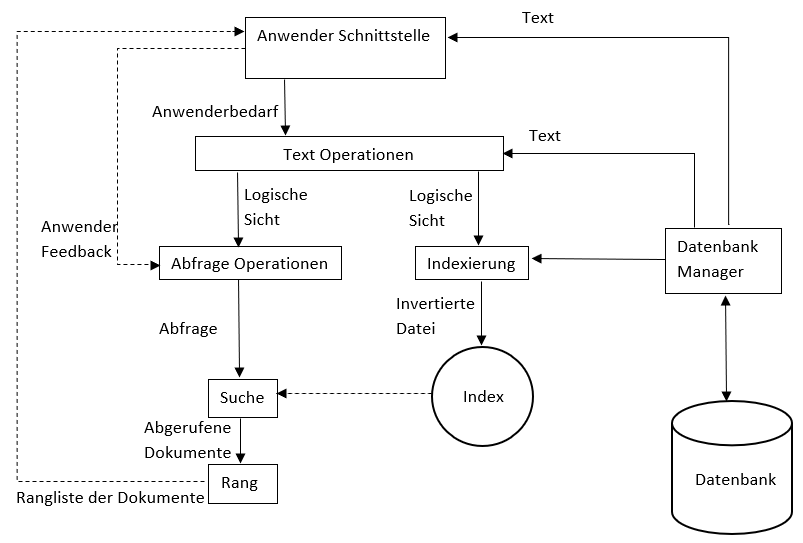
\includegraphics[clip, scale=0.8]{./gfx/Abbildung1_Information_retrievial_Mechanismus.png}
	\caption[Information retrieval Mechanismus]{Der Mechanismus der Informationsrückgewinnung \cite{BRI99}}
	\label{fig:IRMechanismus}
\end{figure}


Die Informationsrückgewinnung wird auf Basis von Modelle durchgeführt. Was das Konzept dieser Modelle ist und wie diese funktionieren wird es zunächst erwähnt.

\subsection{Informationsrückgewinnungsmodelle}
\label{subsec:IRModelle}

Modelle sind charakterisiert durch einen Zweck sowie eine Art und werden definiert als Abbild eines realen Systems oder Problem. Im Fall der Informationsrückgewinnung werden Modelle benutzt um Vereinfachungen zu finden und abstrakt die Zusammenfassung oder die Vernachlässigung von Elemente zu bestimmen. Es bestehen drei Informationsrückgewinnungsmodelle, nämlich das boolesche Modell, das Vektorraummodell und die probabilistischen Modelle.

%\begin{enumerate}
%	\item o
%	\begin{enumerate}
%		\item Das boolesche Modell
 %\item
 \begin{itemize}
 	\item[(1)]Das boolesche Modell 
 
Das boolesche Modell, ist ein Modell, das beruht auf Mengenlehre und boolesche Algebra. Detaillierter ausgedrückt, bei dem booleschen Modell Abfragen können in Form eines booleschen Ausdruckes von Termen formuliert werden, bzw. Terme werden mit den Operatoren UND (Konjunktive Abfrage), ODER (Disjunktive Abfrage) oder NICHT (Negative Abfrage) verbunden. Wegen dem intuitiven Charakter des Konzeptes einer Menge, stellt das boolesche Modell einen leicht zu verstehenden Rahmen für einen gewöhnlichen Benutzer. Des Weiteren Abfragen werden als boolesche Ausdrücke mit präzise Semantik beschrieben. Da das boolesche Modell einfach und formell ist, wurde er in den vergangenen Jahren wahrgenommen und von vielen der frühen kommerziellen bibliografischen Systeme angeeignet. In das boolesche Modell werden Dokumente als eine Menge von Indexbegriffe bezeichnet. Außerdem Indexterme Gewichte sind binär. Das boolesche Modell entscheidet ob ein Dokument relevant oder irrelevant ist für eine gegebene Abfrage. Eine teilweise Übereinstimmung mit dem Dokument wird nicht toleriert. 

\begin{itemize}
	\item[(a)]Das boolesche Modell bietet den Vorteil einfach zu sein und ein sauberer Formalismus in seiner Struktur.
\end{itemize}	
	
	\begin{itemize}
		\item[(b)]Ausdrücke haben eine präzise Semantik, die sie für strukturierte Abfragen geeignet macht, die von "Experten" -Benutzern formuliert werden \cite{CBB13}.
\end{itemize}
	
Es bestehen jedoch auch Nachteile für dieses Modell. Der Hauptnachteil ist, dass die Eigenschaft der totalen Übereinstimmung bei der Informationsrückgewinnung dazu führt, entweder wenige oder zu viele Dokumenten als Ergebnis der Suche zu bekommen. Etwas, das den Anwender die Formulierung guter Abfragen erschwert. Eine Lösung zu dem o. g Nachteil ist die Koordinationsstufe. Mit der Koordinationsstufe können Aussagen aus atomaren Aussagen nichtbinäre Werte haben, bzw. Ranking Dokumente über die reale Linie \cite{MEL15}. Das heißt die binäre Werte des booleschen Modells kein Dokumentenranking ermöglichen bei abwesender Koordinationsstufe.

Die Koordinationsstufe ist ein Maß für den Grad zu dem jedes zurückgegebene Dokument der Abfrage entspricht \cite{MEL15}. Diese stellt eine Punktzahl für das Ranking der Dokumente bereit. Dieses Ranking ermöglicht es dem Benutzer eine Entscheidung über die Menge der zu prüfenden Dokumente zu treffen und gibt dem System die Möglichkeit, den Dokumentenwert, der nach unten gerankt ist, von der Liste abzuschneiden. Die Kalkulation der Koordinationsstufe erfolgt durch die Transkription einer booleschen Abfrage in Konjunktive normale Form (KNF), bzw. durch die Konjunktionsoperator gebundenen Propositionen Liste. Jeder dieser Propositionen präsentiert sich als Disjunktionen von Atom Vorschläge. Die Koordinationsstufe eines Dokuments entspricht die Anzahl der Vorschläge, aus denen eine KNF durch das Dokument zusammengesetzt ist \cite{MEL15}. 

Bei der booleschen Informationsrückgewinnung wird die Gewichtung von Termen nicht bestimmt. Es ergibt sich infolgedessen zu kleine oder zu große Ausgabe \cite{BRI99}]. Wegen diesem Problem wird das boolesche Model in moderne Informationsrückgewinnung nicht mehr eingesetzt. Eine Alternative ist die Erweiterung des booleschen Modells um die Funktionalität von teilweise Übereinstimmung und Begriffsgewichtung. Um die zukünftige Berücksichtigung der variablen Größe zu ermöglichen, wurde eine Variation der Koordinationsstufe dessen Name gewichtete Koordinationsstufe ist, eingesetzt. Bei der gewichteten Koordinationsstufe erfolgt die Zuweisung eines anderen Gewichts abhängig vom Vorschlag, anstatt der Zuweisung konstantes Gewicht zu jedem vom Dokument wahr gemachter Vorschlag (?Satz Formulierung \cite{MEL15} S8??). 

Andere Erweiterungen des booleschen Modells unterstützen die Informations-Nähe und Distanz. Mit diesen Erweiterungen kann spezifiziert werden, ob zwei Begriffe in einer Abfrage in einem Dokument nahe beieinander erscheinen dürfen. Es ist möglich die Nähe zu messen durch Begrenzung der Anzahl von dazwischenliegenden Wörtern oder durch Referenzieren auf eine strukturelle Einheit wie ein Satz oder ein Paragraph (Rock NEAR Roll) \cite{CBB13}.

	 \item[(2)]Das Vektorraummodell 
	
Das Vektorraummodell wird charakterisiert durch den Begriff Ähnlichkeit. Um den grenzenden Aspekt der binären Gewichtseinheiten zu überwinden, bietet das Vektorraummodell einen Rahmen, bei dem die teilweise Abstimmung toleriert wird. Diese teilweise Übereinstimmung erfolgt durch die Zuweisung nicht binäre Gewichtseinheiten zu Indexbegriffe in Abfragen und Dokumenten. Die Begriffsgewichte berechnen den Ähnlichkeitsgrad von jedem Dokument, das gespeichert ist im System und die Anwenderabfrage. Die Berücksichtigung der nur teilweise mit Abfragebegriffen übereinstimmende Dokumente erfolgt beim Ähnlichkeitsgrad durch das Sortieren in absteigender Reihenfolge der Dokumente, die abgerufen wurden. Was sich daraus ergibt ist eine viel genauere Ranglisten-Antwortmenge als die Dokumentenantwortmenge, die mit dem booleschen Modell abgerufen ist. Das Vektorraummodell bewertet das Ähnlichkeitsgrad eines Dokuments in Bezug auf die Abfrage als die Korrelation zwischen zwei Vektoren. Die Quantifikation dieser Korrelation erfolgt beispielsweise durch den Kosinus des Winkels zwischen diesen zwei Vektoren \cite{BRI99}. Anstatt eine Vorhersage über die Relevanz eines Dokuments durchzuführen, das Vektorraummodell geht mit der Klassifizierung der Dokumente entsprechend ihrem Ähnlichkeitsgrad mit der Abfrage vor. Der Abruf eines Dokuments erfolgt dann nur wenn die Bedingung der teilweisen Übereinstimmung erfüllt ist. Die Festlegung eines Schwellenwertes für Ähnlichkeit ist beispielsweise möglich, und den Abruf der Dokumente mit einem Ähnlichkeitsgrad über diesem Schwellenwert ist machbar. Die Berechnung einer Rangliste ist möglich nur wenn die Indexbegriffsgewichte erhalten sind. Diese Indexbegriffsgewichte werden erhalten durch welche begriffsgewichte Techniken, die einen Bezug auf die Clustering-Techniken unterstützende Grundprinzipien.

Die Clustering-Techniken werden wie folgend beschrieben. Ein einfacher Clusteralgorithmus hat als Ziel die Trennung einer Sammlung S von Objekten in zwei Mengen, mit gegebener Sammlung S von Objekten und einer vagen Beschreibung einer Menge M: eine Menge, die Objekte mit Bezug auf die Menge M enthält und eine andere bestehend aus nicht mit der Menge M verwandte Objekte. Die Bedeutung von vage Beschreibung ist, dass keine vollständige Informationen vorhanden sind, um die Entscheidung über anwesende Objekte in der Menge M zu treffen. Es ist möglich für anspruchsvollere Cluster-Algorithmen die Trennung von Objekte einer Sammlung in verschiedene Cluster nach ihren Eigenschaften zu bestreben. Bei einem Clusterproblem kommen zwei Hauptprobleme in Frage, nämlich die muss Ermittlung von Merkmale, die besser beschrieben werden von den Objekten, erfolgen und die Ermittlung von Merkmale, die die Objekte in der Menge M besser von den übrigen Objekten in der Sammlung S differenzieren. Das eine Merkmal setzt eine Quantifizierung der Intra-Cluster-Ähnlichkeit frei und das andere Merkmal erlaubt die Quantifizierung der Ungleichheit zwischen den Clustern. 

Die Quantifizierung in die Intra-cluster-Ähnlichkeit erfolgt durch die Messung der Rohhäufigkeit eines Ausdrucks innerhalb eines Dokuments. Die Bezeichnung von so eine Begriffshäufigkeit heißt Faktor und die Begriffshäufigkeit misst wie gut die Beschreibung des Dokumenteninhalts ist. Die Quantifizierung der Ungleichheit zwischen den Clustern erfolgt durch Messung der Umkehrungshäufigkeit eines Ausdrucks unter den Dokumenten in der Sammlung. Laut \cite{BRI99} das Vektorraummodell bietet die folgenden Vorteile an:

	\begin{itemize}
	\item[(a)]Sein Begriffsgewichtungsschema verbessert die Suchleistung.
\end{itemize}
	\begin{itemize}
	\item[(b)]Seine Strategie der teilweisen Übereinstimmung ermöglicht das Abrufen von Dokumenten, die den Abfragebedingungen angenähert sind.
\end{itemize}
	\begin{itemize}
	\item[(c)]Die Cosinus-Rangliste-Formel sortiert die Dokumente nach ihrem Ähnlichkeitsgrad mit der Suchanfrage
\end{itemize}
	
	Beim Vektorraummodell besteht auch einen Nachteil, nämlich, dass die Index Begriffe als voneinander unabhängig gelten. Die mögliche Beeinträchtigung der Gesamtleitung erfolgt aufgrund der wahllosen Anwendung von Indexbegriffe auf alle Dokumente in der Sammlung \cite{BRI99}.  

	\item[(3)]Die probabilistischen Modelle 

Mit den probabilistischen Modellen werden Informationsrückgewinnungsprobleme mithilfe der Wahrscheinlichkeitstheorie bestimmt. Diese werden benötigt, um das Problem der schwierigen Anwendung des booleschen Modells in Informationsrückgewinnungsaufgaben zu überwältigen. Ein Beispiel von Probleme wäre fehlendes Ranking für Forscher oder fehlendes oder überlastetes Output für den Endbenutzer \cite{MEL15}. Mit dem Vektorraummodell konnte durch Ranking die Verbesserung der Benutzererfahrung erfolgen. Jedoch fehlt immerhin die Ermittlung offenen linearen Koeffizienten. Die probabilistischen Modelle unterstützen ein System dabei die Dokumentdarstellung auf Relevanz zu prüfen und hilft mit Prinzipien bei der Bereitstellung und Verwendung von Gewichte der Koordinationsstufe. Probabilistische Modelle umfassen die Wahrscheinlichkeits-Ranking-Prinzip, das binäre Unabhängigkeitsmodell \cite{MRS08}, Sprachmodelle, das Relevanz Modell \cite{MEL15}. Bevor das Thema des Wahrscheinlichkeits-Ranking-Prinzips behandelt wird, ist es wichtig das Thema Wahr-scheinlichkeitstheorie zu besprechen.

\textbf{Wahrscheinlichkeitstheorie} \cite{MRS08}: Diese ist ein Feld der Stochastik, wo zufällige Ereignisse beschrieben und modelliert werden. Sie beginnt mit als Mengen aufgefasste und Wahrscheinlichkeiten zugeordnete Ereignisse. Die Wahrscheinlichkeiten in diesem Fall entsprechen reelle Zahlen zwischen 0 und 1. gegeben werden zwei Variablen A und B, die Ereignisse Repräsentieren, wobei die Wahrscheinlichkeit für die jeweiligen Ereignisse 0≤ P (A) ≤ 1 und  0 ≤ P (B) ≤ 1 abgefragt wird, da es unsicher ist ob, diese Variablen wahr sind in der reellen Welt. Das gemeinsame Ereignis der beiden Ereignisse wird durch die gemeinsame Wahrscheinlichkeit P (A, B) ausgedrückt. Der Ausdruck P(A|B) bedeutet die Wahrscheinlichkeit des Ereignisses A beim Auftritt des Ereignisses B. Die Kettenregel liefert die grundlegen Beziehung zwischen Kettenregel und die bedingte Wahrscheinlichkeit: 
%\begin{center}
%	P(A|B)=P(A ∩ B)=P(A|B)P(B)=P(B│A)P(A).
%\end{center} 

\textbf{Teil mit Formeln muss noch hinzugefügt werden (wurde im Dokument Masterthesis\_Mpessa.doc 
	rot markiert am 10.06.2018)} 

\textbf{Wahrscheinlichkeits-Ranking-Prinzip (WRP):} Wenn die Antwort eines Referenzabrufsystems auf jede Anfrage eine Rangfolge der Dokumente in der Sammlung ist, in der Reihenfolge der abnehmenden Wahrscheinlichkeit der Relevanz für den Benutzer, der die Anfrage eingereicht hat, werden die Wahrscheinlichkeiten so genau wie möglich auf der Grundlage der Daten geschätzt dem System für diesen Zweck zur Verfügung gestellt wird, ist die Gesamteffektivität des Systems für seinen Benutzer die beste, die auf der Grundlage dieser Daten erhältlich ist [MEL15]. In einem einfachsten binären Fall des Wahrscheinlichkeits-Ranking-Prinzips, dessen Name 1/0 Verlust (engl. 1/0 loss) ist, bestehen keine Wiederauffindungskosten oder andere Versorgungssorgen zur unterschiedlichen Gewichtung von Fehler oder Aktionen. Das Prinzip dieses Falls ist einfach so, dass ein Punkt verloren wird, wenn ein nicht relevantes Dokument zurückgegeben wird oder ein relevantes Dokument nicht zurückgegeben wird. Gezielt wird die Rückgabe der bestmöglichen Ergebnisse als oberste Dokumente, die für den Nutzer wählbar sind. Nach dem Wahrscheinlichkeits-Ranking-Prinzip, die Einordnung der Dokumente muss in absteigender Reihenfolge erfolgen. Falls es um die Rückgabe einer Reihe von Abrufergebnisse anstatt einer Bestellung geht, die Bayes Optimale Entscheidungsregel minimiert das Verlustrisiko beim Zurückgeben von eher relevante als nicht relevante Dokumente. Das WRP ist wichtig, dass es verbindet der prinzipielle Ansatz zum Ranking und den Effektivitätsmaßen. Die Risiken, die im WRP sind probabilistische Definitionen von Rückruf oder Abfallquote. Ob die Maximierung des Rückrufs im Falle einer gegebenen maximal tolerierten Abfallquote relevant ist, wird es determiniert bei der Maximierung der Wahrscheinlichkeit Mithilfe dieser probabilistischen Sichtweise. Das WRP verweist auf die Optimierung der Wiedergewinnungseffektivität sobald der Rückruf für jedes feste Abfallquote-Kosten maximal wird. Das WRP kann auch mit Rückholkosten umgesetzt werden, wo die Modellierung der Differenzkosten von Falschpositiven und Falschnegativen durchgeführt wird.

\textbf{Das binäre Unabhängigkeitsmodell[MRS08]:}Traditionell erfolgt die Anwendung die-ses Modells mit dem WRP. Durch Einführung einfacher Annahmen, ermöglicht das binäre Unabhängigkeitsmodell das Schätzen einer Wahrscheinlichkeitsfunktion zu konkretisie-ren. Binär bedeutet auch boolesch, wobei die Darstellung von Dokumente und Abfragen erfolgt als binäre Begriffsanfall Vektoren. Das heißt die Darstellung eines Dokuments erfolgt durch einen Vektor, der das Wert 1 hat Falls der Begriff im Dokument vorhanden ist oder hat das Wert 0 Falls der Begriff nicht vorhanden ist im Dokument. Das Wort „Unabhängigkeit“ drückt das unabhängige Vorkommen von Begriffe in Dokumenten aus. Die Erkennung einer Assoziation zwischen Begriffe bestehen bei dem Modell nicht. Trotz ihre Unkorrektheit, bietet diese Annahme befriedigende Ergebnisse und entspricht die Annahme von Naive-Bayes-Modellen. Diese Annahme ist auch gleichwertig mit einer Annahme des Vektorraummodells, wo jeder Ausdruck eine zu allen anderen Begriffen orthogonale Dimension entspricht. Die Verfeinerung des Informationsbedarfs von Benutzer erfolgt durch die Anzeige einer Reihe von Ergebnisse. Für eine präzise probabilistische Suchstrategie soll die Abschätzung des Beitrags zur Relevanz von Begriffe in Dokumenten erfolgen. Im binäre Unabhängigkeitsmodell erfolgen die Ableitung einer Ranking-Funktion für Abfragebegriffe, sowie die theoretischen und praktischen Wahrscheinlichkeitsschätzungen. Eine Erweiterung, dessen Name Baumabhängigkeitsmodell ist, versucht die Modellierung von Abhängigkeiten erster Ordnung zwischen Begriffe durch die Verwendung[MET11] .

\textbf{Sprachmodelle \cite{MEL15}:}

\textbf{Das Relevanz Modell \cite{MEL15}:}


Probability theory and ranking, binary independance model


\end{itemize}

\subsection{Web Informationsrückgewinnung}
\label{subsec: WebIR}


